%@ Subject: Elementary Probability
\addpoints

\question[15] Suponga que un día despierta con fuerte dolor de cabeza, síntoma que atribuye a una gripe común. 

Revisando reportes de organismos de salud,  indican que el $80\%$ de las personas con gripe común presentan dolor de cabeza como uno de sus síntomas.

Otra información relevante es que la prevalencia de la gripe común es de un $10\%$. Además que la afección del dolor de cabeza es de un $8.1\%$ en la población.

\noaddpoints
\begin{parts}
\part[5] Defina sucesos e identique las probabilidades. 
\part[5] Determine la probabilidad de tener gripe común dado que sufre de dolor de cabeza.
\part[5] Determine la probabilidad de no tener gripe dado que no sufre de dolor de cabeza.
\end{parts}

\begin{solution}
Sintetizando la información del enunciado tenemos

\begin{center}
% Set the overall layout of the tree
\tikzstyle{level 1}=[level distance=3.5cm, sibling distance=3.5cm]
\tikzstyle{level 2}=[level distance=3.5cm, sibling distance=2cm]

% Define styles for bags and leafs
\tikzstyle{bag} = [text width=4em, text centered]
\tikzstyle{end} = [circle, minimum width=3pt,fill, inner sep=0pt]

% The sloped option gives rotated edge labels. Personally
% I find sloped labels a bit difficult to read. Remove the sloped options
% to get horizontal labels. 
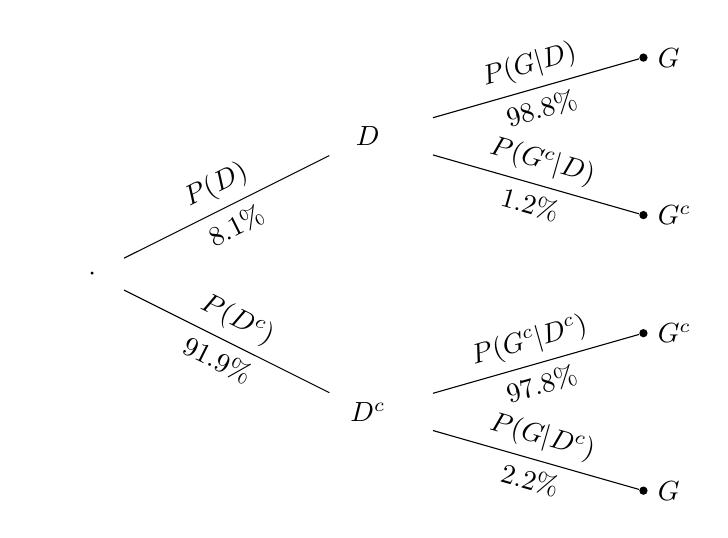
\begin{tikzpicture}[grow=right, sloped]
\node[bag] {$\cdot$}
    child {
        node[bag] {$D^c$}        
            child {
                node[end, label=right:
                    {$G$}] {}
                edge from parent
                node[above] {$\mathbb{P}(G|D^c)$}
                node[below]  {$2.2\%$}
            }
            child {
                node[end, label=right:
                    {$G^c$}] {}
                edge from parent
                node[above] {$\mathbb{P}(G^c|D^c)$}
                node[below]  {$97.8\%$}
            }
            edge from parent 
            node[above] {$\mathbb{P}(D^c)$}
            node[below]  {$91.9\%$}
    }
    child {
        node[bag] {$D$}        
        child {
                node[end, label=right:
                    {$G^c$}] {}
                edge from parent
                node[above] {$\mathbb{P}(G^c|D)$}
                node[below]  {$1.2\%$}
            }
            child {
                node[end, label=right:
                    {$G$}] {}
                edge from parent
                node[above] {$\mathbb{P}(G|D)$}
                node[below]  {$98.8\%$}
            }
        edge from parent         
            node[above] {$\mathbb{P}(D)$}
            node[below]  {$8.1\%$}
    };
\end{tikzpicture}
\end{center}

Alternativamente, se puede establecer el diagrama de árbol alternando los eventos, esto es:

\begin{center}
% Set the overall layout of the tree
\tikzstyle{level 1}=[level distance=3.5cm, sibling distance=3.5cm]
\tikzstyle{level 2}=[level distance=3.5cm, sibling distance=2cm]

% Define styles for bags and leafs
\tikzstyle{bag} = [text width=4em, text centered]
\tikzstyle{end} = [circle, minimum width=3pt,fill, inner sep=0pt]

% The sloped option gives rotated edge labels. Personally
% I find sloped labels a bit difficult to read. Remove the sloped options
% to get horizontal labels. 
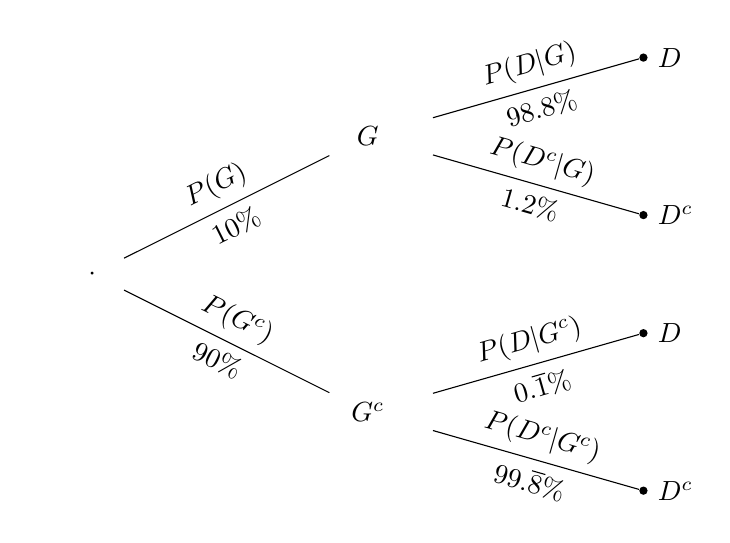
\begin{tikzpicture}[grow=right, sloped]
\node[bag] {$\cdot$}
    child {
        node[bag] {$G^c$}        
            child {
                node[end, label=right:
                    {$D^c$}] {}
                edge from parent
                node[above] {$\mathbb{P}(D^c|G^c)$}
                node[below]  {$99.\overline{8}\%$}
            }
            child {
                node[end, label=right:
                    {$D$}] {}
                edge from parent
                node[above] {$\mathbb{P}(D|G^c)$}
                node[below]  {$0.\overline{1}\%$}
            }
            edge from parent 
            node[above] {$\mathbb{P}(G^c)$}
            node[below]  {$90\%$}
    }
    child {
        node[bag] {$G$}        
        child {
                node[end, label=right:
                    {$D^c$}] {}
                edge from parent
                node[above] {$\mathbb{P}(D^c|G)$}
                node[below]  {$1.2\%$}
            }
            child {
                node[end, label=right:
                    {$D$}] {}
                edge from parent
                node[above] {$\mathbb{P}(D|G)$}
                node[below]  {$98.8\%$}
            }
        edge from parent         
            node[above] {$\mathbb{P}(G)$}
            node[below]  {$10\%$}
    };
\end{tikzpicture}
\end{center}



Podemos definir los eventos del siguiente modo:\\

D: \{ La persona que presenta dolor de cabeza. \}\\

G: \{ La persona que presenta gripe común. \}\\


Las probabilidades asociadas son:

\begin{align*}
\mathbb{P}(D)&=0.081\\
\mathbb{P}(D^c)&=1-0.081=0.919\\
\mathbb{P}(G)&=0.1\\
\mathbb{P}(G^c)&=1-0.1=0.9\\
\mathbb{P}(D|G)&=0.8\\
\mathbb{P}(D^c|G)&=0.2
\end{align*}

Por la definición del teorema de Bayes y la información que podemos obtener del enunciado, tenemos que:

$$\mathbb{P}(G|D)=\frac{\mathbb{P}(D|G) \mathbb{P}(G)}{\mathbb{P}(D)} =\dfrac{0.8*0.1}{0.081}=0.988 $$
y,
$$\mathbb{P}(G^c|D)=1-\mathbb{P}(G|D)=0.012$$

Además sabemos que:

$$\mathbb{P}(G^c)= \mathbb{P}(G^c|D)\mathbb{P}(D) + \mathbb{P}(G^c|D^c)\mathbb{P}(D^c)$$

Así,

$$0.9=0.012*0.081 + \mathbb{P}(G^c|D^c)*0.919$$

Finalmente,

$$\mathbb{P}(G^c|D^c)=(0.9-0.012*0.081)/0.919=0.978$$

\end{solution}